\section{Introduction}

In February 2022, FromSoftware released Elden Ring: the highly anticipated next installment of the amazingly popular franchise, Dark Souls. Boasting an impressive 57 hours of content to reach the end credits, it is entirely unexpected that six months later, the game was completed in just under four minutes — without cheats of any kind. The people responsible for this achievement are known as speedrunners: players that aim to complete a videogame as quickly as possible without cheating. 

This style of playing games has become a sensation within the entertainment and videogame industries, and has consequently created many online communities where players gather to compete and collaborate with each other. The largest of these communities is speedrun.com, a platform that supports over 1.5 million of these players. Viewing these online communities from the perspective of machine learning and data science, they are a heretofore unexplored source of user behavioural data. Therefore, this dissertation aims to investigate the user behaviour and game choices of users on the largest community, speedrun.com, using artificial intelligence and data science.

\begin{figure}[h]
    \centering
    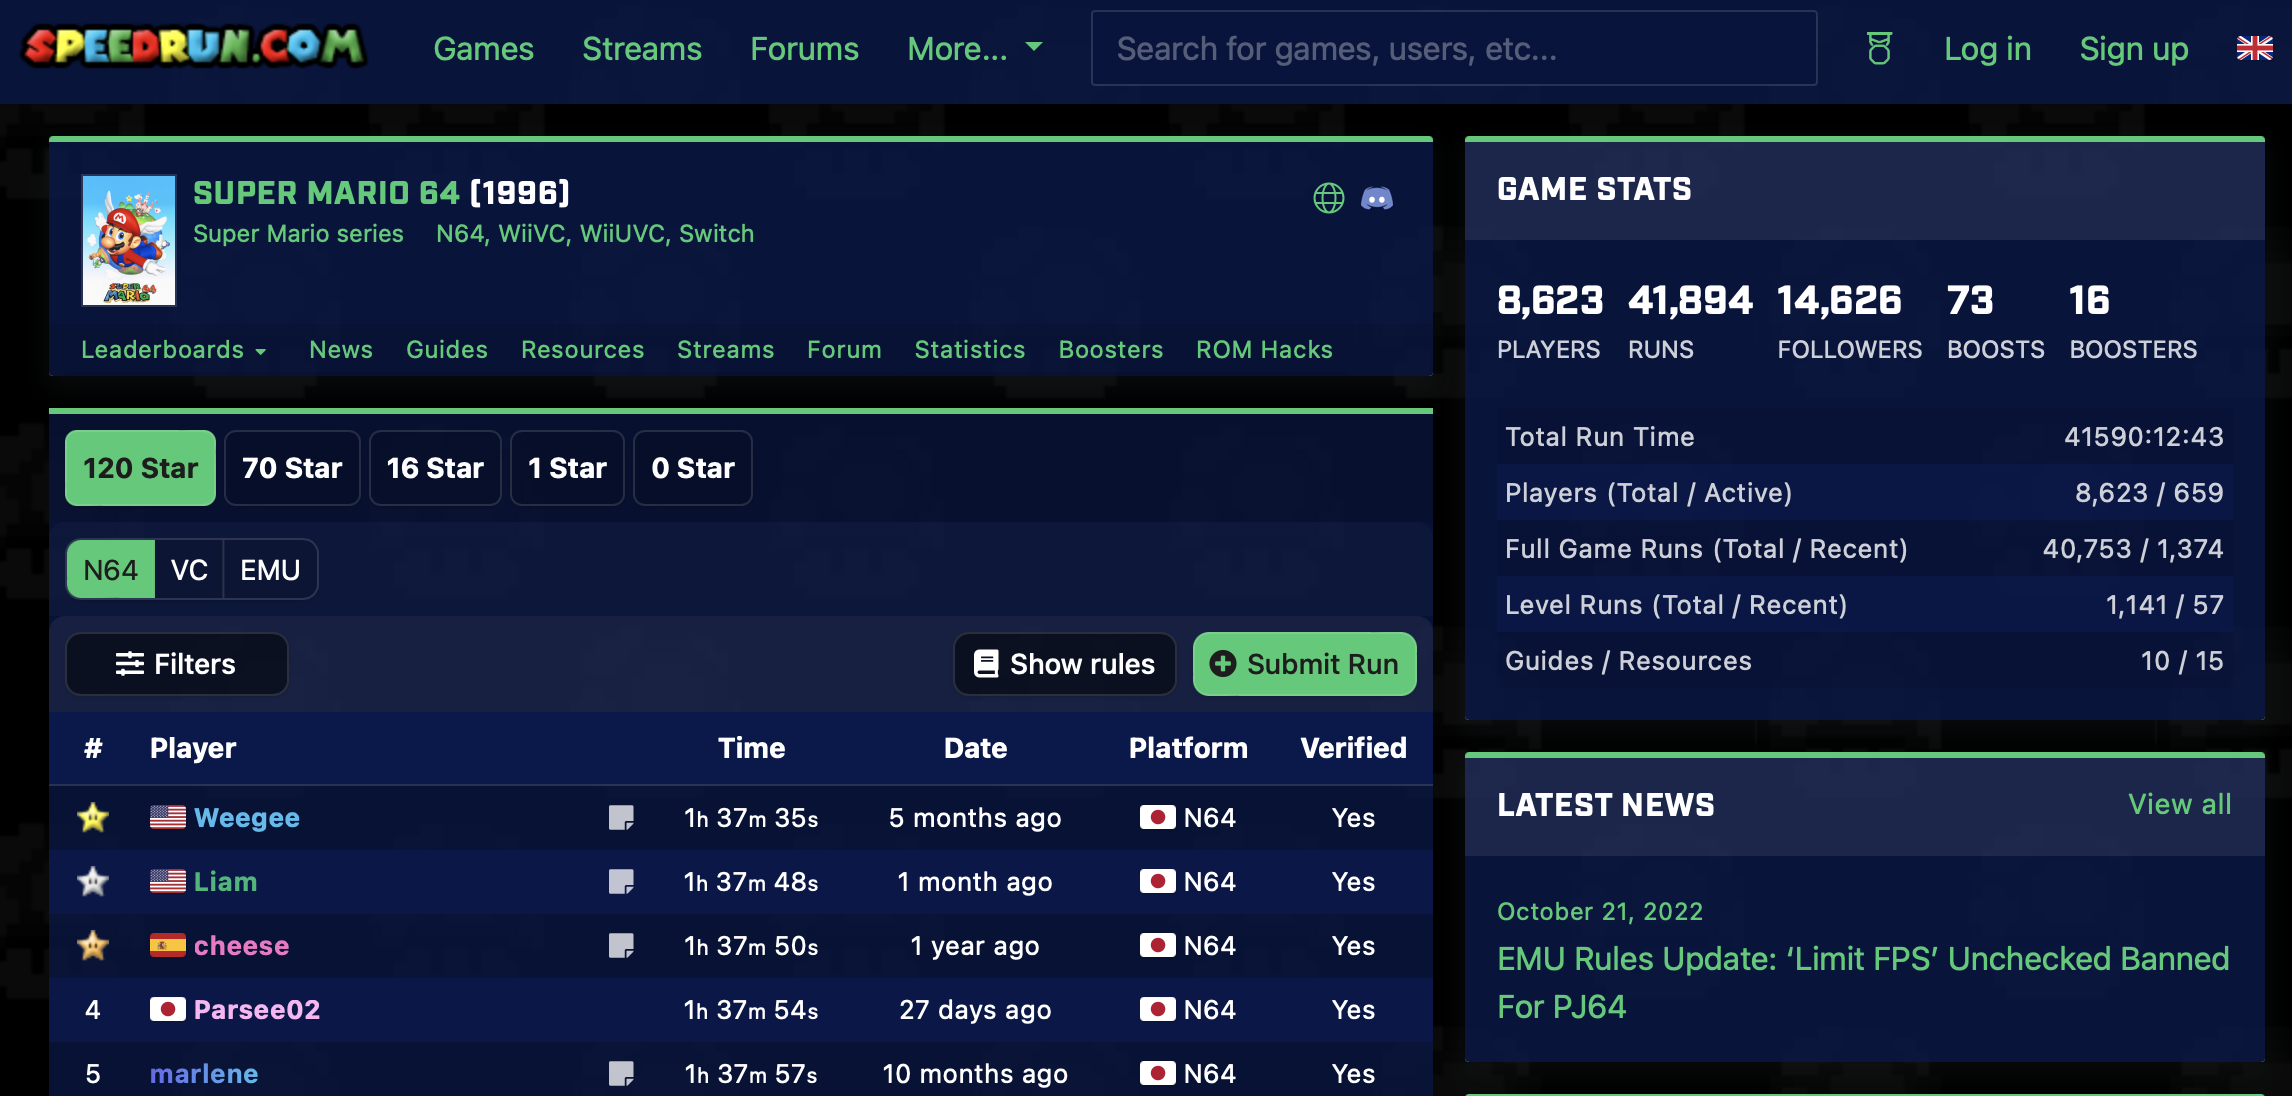
\includegraphics[width=0.8\linewidth]{images/sm64_cropped.png}
    \caption{The leaderboard page for Super Mario 64's 120 star category, filtered by runs on the N64.}
    \label{fig:my_label}
\end{figure}

\vspace{-5pt}
\subsection{Motivation}

There is a broad literature of analysing social networks with data science and machine learning methods. Methods such as community detection and recommendation systems are designed to investigate and provide a practical application of user behavioural data. However, speedrunning has not typically been the subject of machine learning methods. Current literature focuses on elucidating the ethos and principles behind the practice of speedrunning, rather than data analysis \cite{Hemmingsen, ScullyBlaker, EscobarLamanna}. Previous attempts at analysis have focused on the evolution and growth of speedrunning community, rather than understanding the user's behaviour \cite{OrtizSanchez}.


The videogame industry is currently worth approximately \$200 billion, more than all other types of media combined \cite{pwc_outlook}. User behaviour analysis, such as community detection and recommendation systems, provide insight on the trends and demands of the videogame community \cite{Tang2010CommunityDA}. Publishers and developers may then use these insights to make data-driven decisions.


This project aims to contribute to the wider literature by analysing the user behaviour on speedrun.com in an attempt to understand \textit{why} users choose the games they play. This will be partly determined via community detection methods to identify the similarities between users on speedrun.com. Recommendation systems will help determine if this data is suitable for identifying patterns in user behaviour.

\subsection{Aims and Objectives}

The aim of this project is to study the users and games of speedrun.com. Specifically, to investigate and understand the behaviour of users on speedrun.com, and to determine patterns in the choice of games that users play. Additionally, the project aims to make speedrunning data available to enable further research in this topic. This project uses machine learning methods to cluster and compare user behaviour data to determine if user behaviour can be characterised. Online version control systems are used curate and distribute the data source to encourage further research.


There are a few objectives that are necessary to satisfy the aims of the project. These objectives are formatted as research questions, that help structure the results and discussion in this dissertation:

\begin{enumerate}
    \item Are there communities of users and games on speedrun.com? If users and games are clustered in distinct communities, then community detection methods will be able to identify these communities accurately. 
    \item What do the users and games in each community have in common? If the features of both users and games are consistent in an entire community, then different patterns of behaviour can be identified in each community.
    \item Can a game recommendation system be created using speedrunning data? If user preferences can be determined, then the games that users may play will be determined using user-user or game-game similarity.
    \item Are game recommendation systems using this data accurate? Moreover, what methods of recommendation perform better? If a game recommendation system has a reasonable accuracy, then different clusters of users will be determined from their game preferences.
    \item What do games and users on speedrun.com look like? If the features of users and games are analysed, then both can be characterised and contribute to understanding the overall community of speedrun.com.
    \item Can this project produce a publishable data source for future investigation? If the data can be structured to enable distribution, will this entice further investigation into the subject of speedrunning?
\end{enumerate}

These objectives will be met if the research questions can be answered and accompanied with sufficient evidence. First, a list of communities and the trends within the games and users of each community must be produced. Likewise, the recommendation engine must reach a satisfactory accuracy level and produce meaningful recommendations. Finally, the data used in this research must be published online and available for download.


First, the report provides the necessary context to understand the current literature surrounding speedrunning, community detection, and recommendation systems. This is followed by the Design chapter, which describes the resources used and created to ensure the success of the project. The fourth chapter describes the specific implementation of the systems described in the design section, and discusses how these implementations are evaluated and tested. The results are presented and discussed in the fifth and sixth chapters respectively. To conclude, the limitations of the report are discussed, and further avenues for research are proposed.